%%%% Dokumentklassen %%%%

\documentclass[a4paper,11pt,fleqn,dvipsnames,twoside,openany]{memoir} 	% Openright åbner kapitler på højresider (openany begge)


%%%% PACKAGES %%%%

%% Oversættelse og tegnsætning %%
\usepackage[utf8]{inputenc}					% Input-indkodning af tegnsæt (UTF8)
\usepackage[danish]{babel}					% Dokumentets sprog
\usepackage[T1]{fontenc}					    % Output-indkodning af tegnsæt (T1)
\usepackage{ragged2e,anyfontsize}			% Justering af elementer
\usepackage{fixltx2e}						% Retter forskellige fejl i LaTeX-kernen

\usepackage{lastpage}						% Total antal sider opdateres automatisk ved \pageref{LastPage}
																			
%% Figurer og tabeller (floats) %%
\usepackage{graphicx} 						% Håndtering af eksterne billeder (JPG, PNG, EPS, PDF)
\usepackage{multicol}         	            	% Muliggør output i spalter
\usepackage{rotating}						% Rotation af tekst med \begin{sideways}...\end{sideways}
\usepackage{xcolor}							% Definer farver med \definecolor. Se mere: http://en.wikibooks.org/wiki/LaTeX/Colors
\usepackage{flafter}						% Sørger for at floats ikke optræder i teksten før deres reference
\let\newfloat\relax 						% Justering mellem float-pakken og memoir
\usepackage{float}							% Muliggør eksakt placering af floats, f.eks. \begin{figure}[H]

%% Matematik mm. %%
\usepackage{amsmath,amssymb,stmaryrd} 		% Avancerede matematik-udvidelser
\usepackage{mathtools}						% Andre matematik- og tegnudvidelser
\usepackage{textcomp}                 		% Symbol-udvidelser (fx promille-tegn med \textperthousand)
\usepackage{rsphrase}						% Kemi-pakke til RS-saetninger, fx \rsphrase{R1}
\usepackage[version=3]{mhchem} 				% Kemi-pakke til flot og let notation af formler, f.eks. \ce{Fe2O3}
\usepackage{siunitx}						% Flot og konsistent præsentation af tal og enheder med \si{enhed} og \SI{tal}{enhed}
\sisetup{output-decimal-marker = {,}}		% Opsætning af \SI (DE for komma som decimalseparator) 

%% Referencer og kilder %%
\usepackage[danish]{varioref}				% Muliggør bl.a. krydshenvisninger med sidetal (\vref)
\usepackage{natbib}							% Udvidelse med naturvidenskabelige citationsmodeller
\usepackage{xr}							    % Referencer til eksternt dokument med \externaldocument{<NAVN>}

%% Misc. %%
\usepackage{listings}						% Placer kildekode i dokumentet med \begin{lstlisting}...\end{lstlisting}
\usepackage{lipsum}							% Dummy text \lipsum[..]
\usepackage[shortlabels]{enumitem}			% Muliggør enkelt konfiguration af lister
\usepackage{pdfpages}						% Gør det muligt at inkludere pdf-dokumenter med kommandoen \includepdf[pages={x-y}]{fil.pdf}	
\pdfoptionpdfminorversion=6					% Muliggør inkludering af pdf-dokumenter, af version 1.6 og højere
\pretolerance=2500 							% Justering af afstand mellem ord (højt tal, mindre orddeling og mere luft mellem ord)


%%%% CUSTOM SETTINGS %%%%

%% Marginer %%
\setlrmarginsandblock{3.5cm}{2.5cm}{*}		% \setlrmarginsandblock{Indbinding}{Kant}{Ratio}
\setulmarginsandblock{2.5cm}{3.0cm}{*}		% \setulmarginsandblock{Top}{Bund}{Ratio}
\checkandfixthelayout 						% Oversætter værdier til brug for andre pakker

%% Afsnitsformatering %%
\setlength{\parindent}{0mm}           		% Størrelse af indryk
\setlength{\parskip}{3mm}          			% Afstand mellem afsnit ved brug af double Enter
\linespread{1,1}							% Linjeafstand

%% Indholdsfortegnelse %%
\setsecnumdepth{subsection}		 			% Dybden af nummererede overskrifter (part/chapter/section/subsection)
\maxsecnumdepth{subsection}					% Dokumentklassens grænse for nummereringsdybde
\settocdepth{subsection} 					% Dybden af indholdsfortegnelsen
		
%% Opsætning af listings %%
\definecolor{commentGreen}{RGB}{34,139,24}
\definecolor{stringPurple}{RGB}{208,76,239}

\lstset{language=Matlab,					    % Sprog
	basicstyle=\ttfamily\scriptsize,		    % Opsætning af teksten
	keywords={for,if,while,else,elseif,		% Nøgleord at fremhæve
			  end,break,return,case,
			  switch,function},
	keywordstyle=\color{blue},				% Opsætning af nøgleord
	commentstyle=\color{commentGreen},		% Opsætning af kommentarer
	stringstyle=\color{stringPurple},		% Opsætning af strenge
	showstringspaces=false,					% Mellemrum i strenge enten vist eller blanke
	numbers=left, numberstyle=\tiny,		    % Linjenumre
	extendedchars=true, 					    % Tillader specielle karakterer
	columns=flexible,						% Kolonnejustering
	breaklines, breakatwhitespace=true,		% Bryd lange linjer
}

%% Navngivning %%
\addto\captionsdanish{
	\renewcommand\appendixname{Appendiks}
	\renewcommand\contentsname{Indholdsfortegnelse}	
	\renewcommand\appendixpagename{Appendiks}
	\renewcommand\appendixtocname{Appendiks}
	\renewcommand\cftchaptername{\chaptername~}		% Skriver "Kapitel" foran kapitlerne i indholdsfortegnelsen
	\renewcommand\cftappendixname{\appendixname~}	% Skriver "Appendiks" foran appendiks i indholdsfortegnelsen
}

%% Kapiteludssende %%
\definecolor{numbercolor}{gray}{0.7}		            % Definerer en farve til brug til kapiteludseende
\newif\ifchapternonum

\makechapterstyle{jenor}{					        % Definerer kapiteludseende frem til ...
  \renewcommand\beforechapskip{0pt}
  \renewcommand\printchaptername{}
  \renewcommand\printchapternum{}
  \renewcommand\printchapternonum{\chapternonumtrue}
  \renewcommand\chaptitlefont{\fontfamily{pbk}\fontseries{db}\fontshape{n}\fontsize{25}{35}\selectfont\raggedleft}
  \renewcommand\chapnumfont{\fontfamily{pbk}\fontseries{m}\fontshape{n}\fontsize{1in}{0in}\selectfont\color{numbercolor}}
  \renewcommand\printchaptertitle[1]{%
    \noindent
    \ifchapternonum
    \begin{tabularx}{\textwidth}{X}
    {\let\\\newline\chaptitlefont ##1\par} 
    \end{tabularx}
    \par\vskip-2.5mm\hrule
    \else
    \begin{tabularx}{\textwidth}{Xl}
    {\parbox[b]{\linewidth}{\chaptitlefont ##1}} & \raisebox{-15pt}{\chapnumfont \thechapter}
    \end{tabularx}
    \par\vskip2mm\hrule
    \fi
  }
}											        % ... her

\chapterstyle{jenor}						        % Valg af kapiteludseende - Google 'memoir chapter styles' for alternativer

%% Sidehoved %%

\makepagestyle{AAU}							        % Definerer sidehoved og sidefod udseende frem til ...
\makepsmarks{AAU}{%
	\createmark{chapter}{left}{shownumber}{}{. \ }
	\createmark{section}{right}{shownumber}{}{. \ }
	\createplainmark{toc}{both}{\contentsname}
	\createplainmark{lof}{both}{\listfigurename}
	\createplainmark{lot}{both}{\listtablename}
	\createplainmark{bib}{both}{\bibname}
	\createplainmark{index}{both}{\indexname}
	\createplainmark{glossary}{both}{\glossaryname}
}
\nouppercaseheads									% Ingen Caps ønskes

\makeevenhead{AAU}{\small ST3PRJ3 Gruppe 2}{}{\leftmark}	% Definerer lige siders sidehoved (\makeevenhead{Navn}{Venstre}{Center}{Hoejre})
\makeoddhead{AAU}{\rightmark}{}{\small ASE}		            % Definerer ulige siders sidehoved (\makeoddhead{Navn}{Venstre}{Center}{Højre})
\makeevenfoot{AAU}{\small \thepage}{}{}						% Definerer lige siders sidefod (\makeevenfoot{Navn}{Venstre}{Center}{Højre})
\makeoddfoot{AAU}{}{}{\small \thepage}						% Definerer ulige siders sidefod (\makeoddfoot{Navn}{Venstre}{Center}{Højre})

\copypagestyle{AAUchap}{AAU}							% Sidehoved for kapitelsider defineres som standardsider, men med blank sidehoved
\makeoddhead{AAUchap}{}{}{}
\makeevenhead{AAUchap}{}{}{}
\makeheadrule{AAUchap}{\textwidth}{0pt}
\aliaspagestyle{chapter}{AAUchap}					% Den ny style vælges til at gælde for chapters
													% ... her
															
\pagestyle{AAU}										% Valg af sidehoved og sidefod


%%%% CUSTOM COMMANDS %%%%

%% Billede hack %%
\newcommand{\figur}[4]{
		\begin{figure}[H] \centering
			\includegraphics[width=#1\textwidth]{billeder/#2}
			\caption{#3}\label{#4}
		\end{figure} 
}

%% Specielle tegn %%
\newcommand{\decC}{^{\circ}\text{C}}
\newcommand{\dec}{^{\circ}}
\newcommand{\m}{\cdot}


%%%% ORDDELING %%%%

\hyphenation{}


%%%% Tilføjelser af min preample %%%%

% Booktabs:
% The booktabs package is needed for better looking tables. 
\usepackage{booktabs}

% Caption:
% For better looking captions. See caption documentation on how to change the format of the captions.
\usepackage[hang, font={small, it}]{caption}

% Hyperref:
% This package makes all references within your document clickable. By default, these references will become boxed and colored. This is turned back to normal with the \hypersetup command below.
\usepackage{hyperref}
	\hypersetup{colorlinks=false,pdfborder=0 0 0}

% Cleveref:
% This package automatically detects the type of reference (equation, table, etc.) when the \cref{} command is used. It then adds a word in front of the reference, i.e. Fig. in front of a reference to a figure. With the \crefname{}{}{} command, these words may be changed.
\usepackage{cleveref}
	\crefname{equation}{formel}{formler}
	\crefname{figure}{figur}{figurer}	
	\crefname{table}{tabel}{tabeller}

% Mine tilføjelser:
\usepackage{units}                        %% Bruges til at gøre fx 1/2 samlet med: \nicefrac{1}{2}.
\usepackage{tabu, longtable}              %% Bruges til tabeller.
\setlength{\tabulinesep}{1.5ex}           %% Definerer linjeafstand i tabeller.
\usepackage{enumerate}                    %% Bruges til lister.
\usepackage{tabto}                        %% Giver mulighed for TAB med fx \tabto{3em}.
\usepackage[hyphenbreaks]{breakurl}       %% Bruges til websiders url'er.
\renewcommand{\UrlFont}{                  %% Definerer url-font.
\small\ttfamily}                          %
\bibliographystyle{unsrt}                 %% Definere bibliografien. Ses til sidst i dokumentet i kapitlet Litteratur.
\usepackage{amssymb} 
\usepackage{pifont}
%\newcommand{\xmark{\ding{55}}			 % Opretter et unchecked mark
\raggedbottom

%\externaldocument[D-]{Dokumentation}

\begin{document}

	
\frontmatter						% Nummereres med romerske tal.
\let\cleardoublepage\clearpage
\begin{titlingpage}
\begin{center}

~ \\[3cm]


\includegraphics[width=0.6\textwidth]{figurer/ASE}~\\[1cm]

\textsc{\LARGE Aarhus School of Engineering}\\[1.5cm]

\textsc{\Large Sundhedsteknologi}\\
\textsc{\Large 3. semesterprojekt}\\[0.5cm]

\noindent\makebox[\linewidth]{\rule{\textwidth}{0.4pt}}\\
[0.5cm]{\Huge Rapport}
\noindent\makebox[\linewidth]{\rule{\textwidth}{0.4pt}}

\end{center}



\textit{Gruppe 2} \newline
Anne Bundgaard Hoelgaard\tab(201404492) \newline
Mette Hammer Nielsen-Kudsk\tab(201408391) \newline
Ditte Heebøll Callesen\tab(201408392) \newline	
Martin Banasik\tab(201408398) \newline	
Albert Jakob Fredshavn\tab(201408425) \newline 
Johan Mathias Munk\tab(201408450) \newline 




\textit{Vejleder:} \newline
Studentervejleder\\
Peter Johansen\\
Aarhus Universitet


\vfill

\begin{center}
{\large 16. december 2015}
\end{center}


\end{titlingpage}

\chapter{Resumé}
Dette projekt beskæftiger sig med blodtryksmåling, hvor der ud fra et blodtrykssignal kan bestemmes en systolisk- og diastolisk værdi, samt en pulsværdi. Formålet er at bygge en hardwaredel, der kan trykændre et analogt signal. Via et filter skal signalet forstærkes og sendes videre igennem en Data Acquisition (DAQ), der kan lave det analoge signal om til et digitalt signal. Herefter skal signalet videre ind i softwaren. Her er formålet at få programmeret en algoritme, der kan detektere en puls samt en systolisk- og diastolisk værdi. Disse systole- og diastoleværdier kan findes ud fra det digitale signal. Signalet bliver observeret fra starttidspunktet, hvor værdien for trykket begynder at vokse, indtil grafen når maksimum. Når værdien igen begynder, kan programmet detektere den højeste værdi, som er den systoliske værdi. Efter maksimum begynder grafen for signalet at falde igen, da trykket bliver mindre, indtil det når det laveste punkt, hvor værdien igen begyndte at stige en smule. 
Dette lavpunkt er værdien for diastolen. Grafen er periodisk og ud fra den systoliske- og diastoliske værdi kan pulsen findes. \\
Herudover skal programmet kunne kalibreres og nulpunktsjusteres når forskeren synes nødvendigt. Projektet er lavet til forskningsbrug og derfor blev det vurderet, at det er nødvendigt for en forsker, at kunne gemme sine målinger. Programmeringen skal derfor også gøre det muligt for forskeren, at kunne gemme sine målinger i en database.  \\
Resultatet for dette projekt viser at det er muligt vha. hardware- og softwaredelen, at måle et blodtryk. Gennem videreudvikling kan det blive muligt at detektere hypertension (Forhøjet blodtryk) og hypotension (Lavt blodtryk) i samme program. Dette ville være nyttigt, hvis projektet i fremtiden skulle bruges til patienter. I projektet er der dog udelukkende blevet arbejdet med måling af blodtryk.

\chapter{Abstract} 
This project has primarily been focused on blood pressure measurement, where systolic- and diastolic values, as well as the pulse, could be determined. The purpose of this project is to construct hardware and software which can manipulate the pressure of an analog signal as well as depict this signal using developed software. By using an analog filter, the analog signal is amplified and sent to a Data Acquisition (DAQ), where the signal will be transformed from an analog signal to a digital signal. This digital signal will afterwards enter a computer, running the software program. Here the purpose of the software is to program an algorithm, which can detect a pulse as well as the systolic- and diastolic values. These two values are found by looking at the visualized signal.  From the beginning of the graph, and until the signal ascends to maximum and falls again. This maximum value is the systolic value. Afterwards the signal will begin to descend until a minimum is reached, where this minimum is the diastolic value. The graph will then slightly climb again and begin a new period. From these systolic- and the diastolic values, the pulse can be found.\\
In addition to the above requirements, the program is able to be calibrated and zero adjusted, whenever the researcher finds it necessary. \\
This project is made for research use and it was therefore decided that a necessity for a researcher, would be to save his measurements in a database. \\
The result of this project shows that it is possible to measure blood pressure through a combination of hardware and software. Through future development it could be possible for the program to detect hypertension (high blood pressure) and hypotension (low blood pressure). This would be useful if the project, in the future, would be used on patients. In this project however, the main goal has exclusively been measurements of blood pressure. 

\begin{vplace}[0.6]
{\large \textit{Gruppemedlemmer}}
\\
\\

\noindent \begin{tabular}{ll}
	\makebox[3.0in]{\hrulefill} & \makebox[1.5in]{\hrulefill}\\
	Albert Jakob Fredshavn  (201408425) & Dato\\[7ex]% adds space between the two sets of signatures
	\makebox[3in]{\hrulefill} & \makebox[1.5in]{\hrulefill}\\
	Ditte Heebøll Callesen  (201408392) & Dato\\[7ex]
	\makebox[3in]{\hrulefill} & \makebox[1.5in]{\hrulefill}\\
	Martin Banasik  (201408398) & Dato\\[7ex]
	\makebox[3in]{\hrulefill} & \makebox[1.5in]{\hrulefill}\\
	Mette Hammer Nielsen-Kudsk  (201408391) & Dato\\[7ex]
	\makebox[3in]{\hrulefill} & \makebox[1.5in]{\hrulefill}\\
	Johan Mathias Munk  (201408450) & Dato\\[7ex]
	\makebox[3in]{\hrulefill} & \makebox[1.5in]{\hrulefill}\\
	Anne Bundgaard Hoelgaard (201404492) & Dato\\[7ex]
	
	
\end{tabular}
\\
{\large \textit{Vejleder}}
\\
\\
\\
\noindent \begin{tabular}{ll}
	\makebox[3.0in]{\hrulefill} & \makebox[1.5in]{\hrulefill}\\
	Peter Johansen & Dato\\[8ex]
\end{tabular}
\end{vplace}

\chapter{Godkendelsesformular}

{\LARGE\textit{Godkendelsesformular}}

{\large Forfattere:}
\\[5ex]


\begin{tabular}{c c}
\centering 
	\makebox[2.0in]{\hrulefill} & \makebox[2.0in]{\hrulefill}\\
	Albert Jakob Fredshavn & Ditte Heebøll Callesen\\[7ex]
	\makebox[2.0in]{\hrulefill} & \makebox[2.0in]{\hrulefill}\\
	Martin Banasik & Mette Hammer Nielsen-Kudsk\\[7ex]
	\makebox[2.0in]{\hrulefill} & \makebox[2.0in]{\hrulefill}\\
	Johan Mathias Munk & Anne Bundgaard Hoelgaard\\[7ex]
	

\end{tabular}

\begin{tabular}{c c c c}
	\textbf{Godkendes af} & Peter Johansen\\[3ex]
	\textbf{Antal sider} & c \\[3ex]
	\textbf{Kunde} & Aarhus Universitet
\end{tabular}\\[8ex]
Ved underskrivelse af dette dokument accepteres det af begge parter som værende kravene til udviklingen af det ønskede system.
\\
\\
\textbf{Dato: } 16/12-2015\\[7ex]

\begin{tabular}{c c}
	\makebox[2.0in]{\hrulefill} & \makebox[2.0in]{\hrulefill}\\
	\centering 
	Kundens underskrift & Leverandørens underskrift
\end{tabular}


%\cleardoublepage	
	
\tableofcontents*                   % Indsætter en indholdsfortegnelse før Indledning.

\mainmatter                         % Her findes de nummererede kapitler modsat \frontmatter og \backmatter. Nummereres med arabiske tal.
\chapter{Ordliste}

\begin{longtabu} to \linewidth{@{}l X[j]@{}}
    Ord &    Forklaring\\
    \toprule\
(F)URPS+ 	&    Et akronym, der repræsenterer en model til klassificering af softwarens kvalitet \\
    GUI		&	Graphical User Interface (Grafisk brugergrænseflade)\\
    VPN		&	Virtual Private Network\\
    DAQ		&	Data acquisition \\
    SysML	&   Systems Modeling Language – sprog til visuel fremstilling af systemer \\
    UML		& Unified modelling language – sprog til oversigtsfremstilling af klasser i programmering \\
    KSS		&	Kommunikation og Samarbejde i Sundhedsvæsnet \\
    BDD 	&	Block Defination Diagram \\
	IBD		& 	Intern Block Diagram \\
	SD		& 	Sekvensdiagram \\
	UML		& 	Unified Modeling Language \\
	ISE 	&	Indledende System Engineering \\
	Hjerteinsufficiens &  Hjertesvigt \\
	DSB		&	Digital Signalbehandling \\
	Hypertension &  Forhøjet blodtryk \\
	Hypotension & Lavt blodtryk \\
	MTTR	&	Mean Time To Restore \\
	MTBF	&	Mean Time Between Failure \\
 
\label{forkort}
\end{longtabu}

\chapter{Indledning}
I dette projekt arbejdes der med blodtryksmålere. Vi har valgt at udarbejde en blodtryksmåler til forskningsbrug. Blodtryksmåleren skal kunne modtage en spænding fra en transducer, nulpunktsjustere og kalibere efter en forskers ønske. Signalet skal vises i en graf, på et display, hvor værdier for puls, systoliske- og diastoliske tryk vises. Her fra forskeren starter og gemmer sine målinger.\\
I kravspecifikationen findes de krav, der er blevet stillet for projektet. Herunder er også de krav, som blev stillet mellem os og vores vejleder.\\
Under systemarkitekturen findes informationer om, hvordan software- og hardwaredelen er opbygget.  I afsnittet integrationstest kan der læses om, hvordan projektet er blevet testet.\\  

\subsubsection{Versionshistorik}

\begin{longtabu} to \linewidth{@{}l l l X[j]@{}}
    Version &    Dato &    Ansvarlig &    Beskrivelse\\[-1ex]
    \midrule
    0.1 &   04-11-2015	&   MHNK  &   Oprettelse af LaTex dokumenter \\
    0.2 &   11-11-2015	&   ABH  &   Udviklingsværktøjer og krav \\
    0.3 &   11-11-2015	&   DHC  &   Metoder \\
    0.4 &   18-11-2015	&   ABH  &   Systembeskrivelse  \\
    0.5 &   19-11-2015	&   DHC  &   Perspektivering - Fremtidigt arbejde \\
    0.6 &   24-11-2015	&   MHNK  &   Blodtryk \\
    0.7 &   24-11-2015	&   AJF  &   Projektgennemførelse og -styring \\
    0.8 &   24-11-2015	&   MM  &   Projektformulering og afgrænsning \\
    1.0 &   01-12-2015	&   MB, MHNK  &   Referencelister i LaTex \\
    1.1 &   02-12-2015	&   MB, MHNK  &   Figurlister i LaTex \\
    1.2 &   02-12-2015	&   MHNK  &   Resume \\
    1.3 &   07-12-2015	&   MHNK  &   Abstract \\
    1.4 &   09-12-2015	&   MHNK  &   Konklusion \\
   
    	
\label{version_Systemark}
\end{longtabu}
\chapter{Projektformulering og afgrænsning}
I daglig klinisk praksis er der ofte behov for kontinuert at monitorere patienters blodtryk, i særdeleshed på intensive afdelinger samt operationsstuer, hvor blodtrykket er en vigtig parameter i monitorering af patienters kardiovaskulære status.


Denne kontinuere monitorering er også nødvendig i forskningsverdenen. Det er i forskerens interesse, at kunne måle blodtrykket når der laves hæmodynamiske undersøgelser. Her skal det være muligt for forskeren at kunne aflæse det diastoliske- og systoliske tryk, pulsen samt få vist en pæn kurve over blodtrykket. Det er målet, at opbygge en prototype, der kan registrere de spændinger, i milivolt (mV), der kommer fra tryktransduceren og analogt forstærke samt filtrere signalet. Dette signal skal derefter konverteres til det digitale domæne. \\
Herfra skal der programmeres en brugergrænseflade, der fremfører disse målinger, samt gør det muligt, for forskeren, at gemme målingen i en database til senere brug. Resultatet bliver derfor et elektronisk kredsløb med forbindelse til et software program.
For at de gemte data kan sammenlignes, kræver det at de alle er blevet gemt med samme forudsætning, dvs. at målingerne er blevet kalibreret og nulpunktsjusteret. Dette bliver håndteret i softwaredelen, hvor beregninger implementeres. Når forskeren kigger på blodtryksgrafen, vil han normalt se på et filtreret signal. I tilfælde af at det er i hans interesse at se på et ufilteret signal, vil dette være muligt, ved et tryk på en knap.

\textbf{MoSCoW \footnote{Metode, der benyttes til at beskrive hvad programmet skal kunne og det der ønskes, men ikke vil ske - Must have, Should have, Could have, og Would like but won't get}}
\\
\textit{Must}
\begin{itemize}
\item Et elektronisk kredsløb, som forstærker signalet fra tryktranduceren og filtrerer det med ét indbygget analogt filter
\item Et program til at vise blodtrykket som funktion af tiden. Programmet skal opfylde en række obligatoriske krav. Det skal kunne:
\begin{itemize}
\item Programmeres i C\#
\item Kunne kalibrere blodtrykssignalet og foretage en nulpunktsjustering
\item Vise blodtrykssignalet kontinuert
\item Kunne gemme de målte data i en database
\item Kunne filtrere blodtrykket i selve programmet via et digitalt filter, som skal kunne slås til og fra (monitor mode = filtreret og afrundet; signaldiagnose mode = råt signal med alle udsving)
\item Afbildning af systolisk/diastolisk blodtryk med tal
\end{itemize}
\end{itemize}
\textit{Should}

\textit{Could}
\begin{itemize}
\item Hardwaredelen skal bestå af ét VEVO Board med indbyggede komponenter

\end{itemize} 
\textit{Would}
\begin{itemize}
\item Alarmering, hvis blodtrykket afviger indbyggede grænseværdier
\item Forskeren skal kunne hente de gemte data ned igen
\end{itemize}

\subsubsection{Ansvarsområder}

Idet gruppens størrelse ikke lægger op til samlet, at arbejde på alle dele samtidig, er projektets ansvarsområder blevet fordelt som følgende:

\begin{longtabu} to \linewidth{@{}l l l X[j]@{}}
    Navn &    Ansvarsområder &    \\[-1ex]
    \midrule
    Ditte Heebøll Callesen &   Hardwaredesign, dokumentation	&    \\
    Albert Jakob Fredshavn &   Hardwaredesign, dokumentation	&    \\
    Martin Banasik         &   Hardwaredesign, dokumentation	&    \\
    Johan Mathias Munk     &   Softwaredesign, algoritmeopbygning, dokumentation &    \\
    Mette Hammer Nielsen-Kudsk &   Softwaredesign, algoritmeopbygning, dokumentation &    \\
   	Anne Hoelgaard    &   Softwaredesign, algoritmeopbygning, dokumentation	&    \\
\label{version_Systemark}
\end{longtabu}

\begin{longtabu} to \linewidth{@{}l l l X[l]@{}}
    Navn &    Skrevet afsnit \\%[-1ex]
    \midrule
    Ditte Heebøll Callesen & Indledning, Metoder, systemarkitektur, problemidentifikation, projektstyring og perspektivering \\
    Albert Jakob Fredshavn &  Projektgennemførelse \\
    Martin Banasik         & Systemarkitektur (hardware) og Opnåede resultater \\
    Johan Mathias Munk     & Projektformulering og afgrænsning  \\
    Mette Hammer Nielsen-Kudsk & Resumé, abstract, Blodtryk, resultater og diskussion og konklusion  \\
   	Anne Hoelgaard   	 	& Krav, Systemarkitektur (software) \\
%\label{version_Systemark}
\end{longtabu}


\chapter{Blodtryk}
\section{Hvad betyder blodtryk?} 
Alle har på et tidspunkt i deres liv fået målt blodtryk, men hvad betyder det egentlig?
Blodtryksmåling er en enkelt undersøgelse, der giver vigtige informationer om blodkarrenes og hjertets tilstand. Blodtryk kan måles både invasivt og ikke-invasivt. Dette projekt omhandler invasivt blodtryksmåling, som er en måling af trykket direkte i en blodåre. 
Blodtrykket måles i enheden millimeter kviksølv (mmHg). Et normalt blodtryk ligger på omkring 120/80 mmHg \cite{Blodtryk}. \\ 
Hjertet pumper iltet blod ud i hele kroppen via arteriesystemet og sørger dermed for tilførslen af ilt og næringssubstanser til alle muskler og organer. De røde blodlegemer (erythrocytterne) er en vigtig bestanddel af blodet. Det er hæmoglobinet i de røde blodlegemer, som binder ilten og sørger for at ilten transporteres frem til vævene i kroppen. Når ilten er afgivet fra blodet til musklerne og andre væv, transporteres blodet tilbage til højre side af hjertet via venesystemet. Det af-iltede blod pumpes af højre hjertepumpekammer ud i lungerne, hvor blodet iltes på ny og derfra strømmer til venstre hjertehalvdel, for igen at blive pumpet ud i kroppen af venstre hjertepumpekammer. \\
Det høje tryk er det systoliske tryk, som kan måles når venstre ventrikel trækker sig sammen. Det diastoliske blodtryk er blodtrykket i hjertets afslapningsfase (diastolen). Når hjertet trækker sig sammen (systolen) skaber det en trykbølge som forplanter sig ud igennem arteriesystemet. Trykbølgen kan identificeres som pulsen, der let kan mærkes f.eks. ved palpation af a. radialis ved håndleddet, hvor man mærker på årene. Trykket i venesystemet er meget lavere end i arteriesystemet, da blodet passivt skal strømme tilbage til højre forkammer, hvor trykket er lavt. \\
Venstre ventrikel pumper iltet blod, under højt tryk, ud i aorta og arterierne. Disse blodårer er derfor tykvæggede og elastiske i modsætning til venerne, der er ganske tyndvæggede, fordi de kun udsættes for et lavt tryk. Hjertet overfører, gennem systolen, energi til arterievæggen, som bruges i den resterende del af hjertets cyklus, til at presse blod gennem karsystemet. 


For at forstå det følgende afsnit introduceres tre vigtige begreber nedenfor: 
\begin{itemize}
\item Væskevolumen, der løber igennem et rør pr. tidsenhed, kaldes for væskestrømmen
\item Distancen, som en væske flytter sig pr. tidsenhed er strømningshastigheden
\item Blodvolumen, der løber gennem et væv pr. tids- og vægtenhed er gennemblødning
\end{itemize}

Der er en trykforskel imellem begyndelsen og slutningen af et rør. Væskestrømmen i røret afhænger af trykforskellen hen over røret og modstanden i røret. Dette kan udtrykkes i følgende ligning som ligner Ohms lov for elektriske kredsløb:

\begin{equation}
V$æ$skestr$ø$m(Q)= \frac{Trykforskel(\Delta P)}{Modstand(R)}
\end{equation}

Drivkraften for væskestrømningen (Q) er trykforskellen $(\Delta P)$ gennem røret. Hjertets kontraktioner gør, at strømmen i røret går fra et højere, til et lavere tryk. 
Modstanden (R) i en arterie er bestemt af bl.a. gnidningsmodstanden mellem arterievæggen og blodet, blodets viskositet og diameteren af arterien. Når blodet løber igennem arterierne, falder trykket efterhånden i blodet. Ved stigende modstand mod væskestrømmen forøges trykfaldet. 
Når modstanden i rørvæggen stiger, formindskes væskestrømningen, hvis trykforskellen samtidig ikke er steget.

Et rørs modstand bestemmes ud fra tre parametre: 

\begin{itemize}
\item Længden af røret
\item Den indre diameter på røret 
\item Viskositeten af væsken
\end{itemize}

Jo kraftigere hjertet pumper, desto større bliver trykforskellen og dermed blodstrømningen. 
Blodkarrets diameter er det, der har størst betydning for modstanden mod blodstrømmen. Hvis blodet presses igennem et snævert kar, er der en større del af blodet, der er tæt på karvæggen og blodet bliver derved bremset af friktionskraft. Modsat, hvis diameteren på karret havde været større, ville en mindre del af blodet være i kontakt med væggen og derved ville det ikke blive bremset lige så meget. Modstanden er derfor mindre og blodstrømningen større, i et stort kar. \\
Blodets viskositet stiger, jo flere røde blodlegemer, der findes i blodet. Jo flere røde blodlegemer, desto højere viskositet. Hvis blodet har en høj viskositet og derved er tyktflydende, så skal der et større tryk til at holde en bestemt væskestrøm \cite{Blodtryk}. 
   
\section{Hypertension} 
Hypertension er en meget almindelig lidelse, ca. 30\% af den danske befolkning har forhøjet arterielt blodtryk \cite{Hypertension}. Derfor er det vigtigt ofte at få målt sit blodtryk, da forhøjet blodtryk ikke kan mærkes og er den vigtigste årsag til hjerte-kar-sygdomme. 
Der er tale om hypertension når blodtrykket er 140/90 mmHg eller højere.
Ved hypertension bliver arbejdsbelastningen af hjertet forøget, da der skal pumpes blod ud af hjertet mod en større modstand i arteriesystemet. \\
Forhøjet blodtryk gør at arbejdsbelastningen bliver større. Derved sker der lige så stille en fortykkelse af muskulaturen i venstre ventrikel, da hjertet skal bruge flere kræfter på at pumpe blodet ud i aorta. 
Det øgede tryk påvirker blodkarrenes belastning, og kan medføre at mindre blodkar kan briste under det høje tryk. Hvis der er tale om blodkar i hjernen kan dette føre til en hjerneblødning. Hypertension er den hyppigste årsag til hjerneblødninger.
Hypertension kan føre til en række andre komplikationer i form af åreforkalkning, hjerteinsufficiens \cite{Hjerteinsufficiens}, akut myokardieinfarkt, hjertekrampe, nyreskader og apopleksi.\\
Forhøjet blodtryk behandles med lægemidler, i form af blodtryksnedsættende medicin (antihypertensiva). Samtidig er non-farmakologiske metoder, som rygestop, motion, reduktion af saltindtagelse, vægttab og reduktion af alkoholforbrug vigtige i behandlingen af hypertension. 

\section{Hypotension} 
Hypotension er, modsat hypertension, et lavt blodtryk, og ikke nær så almindeligt. Der er tale om hypotension når blodtrykket er 90/60 mmHg. Hypotension ses især ved en række alvorlige akutte tilstande som akut myokardieinfarkt, lungeemboli, sepsis eller alvorlige blødninger. Patienten kan i disse situationer være i en livstruende shock tilstand. Lavt blodtryk kan også i sjældne tilfælde forekomme kronisk, især ved sjældne stofskiftesygdomme med nedsat produktion af binyrebarkhormoner \cite{Hypotension}.   
\chapter{Systembeskrivelse}
Med udgangspunkt i projektformuleringen kommer dette projekts endelige system til at bestå af et software og hardware system, der kan tilsluttes et måleobjekt, hvorpå et blodtryk kan måles. Systemet skal kunne implementeres i forskningsmiljøer, hvor en eller flere forskere ønsker at analysere indhentede blodtrykssignaler. Visionen er, at systemet skal være let tilgængeligt og effektivt, hvilket vil komme til udtryk ved, at systemet fungerer stabilt.

I dette projekt realiseres en prototype af systemet. Det vil sige at flere dele af systemet udvikles ud fra forsimplede metoder ift. hvordan det vil være optimalt at implementere dem i virkeligheden. Her tænkes på hardware-, såvel som software-elementer. Hardwaren i prototypen realiseres på et VEVO Board, så det er muligt at tage den med sig, samt er mere holdbar over tid. Softwaren i prototypen består af flere moduler. Disse er opbygget efter principperne i en trelagsmodel, hvilket vil sige, at koden indeholder et database-lag, logik-lag samt præsentations-lag. Dette er valgt for, at skabe et overblik over hvilke dele af software-koden der har ansvaret for de enkelte funktionaliteter i systemet.

Hardwaren består af en forstærker og et filter. Forstærkerens opgave består i at forstærke det analoge signal fra max 11 millivolt til 5 volt. Filtret sørger for at filtrere unødigt støj fra det analog signal. Signalændringen fra måleobjektet til visning af signal på en graf er skitseret herunder. Det skal pointeres at dette kun er en skitse for at skabe overblik, derfor er flere processer i softwaren udeladt af diagrammet. 
\begin{figure}[htb]
	\centering
	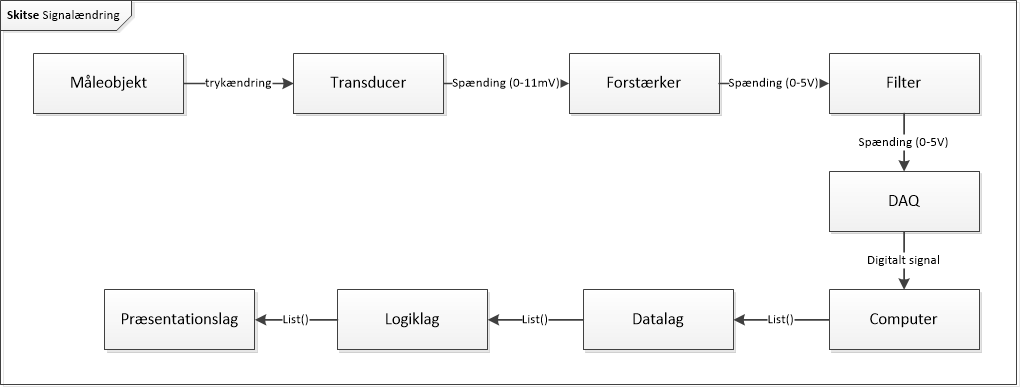
\includegraphics[width=1.0\textwidth]{Figurer/Signalandring}
	\caption{Skitse af signalændring}
	%\label{fig:Skitse der viser signalændring}
\end{figure}
Database-laget består af en lukket database samt indhentningen af blodtrykssignalet fra måleobjektet til transduceren, gennem hardware, inden det rammer software-delen. I den lukkede database gemmes det indhentede blodtrykssignal i en tabel. Signalet gemmes med et tidsstempel, samt under et autogenereret Id, sammensat med det forsøgsnavn som forskeren indtaster på brugergrænsefladen ved begyndelsen af en måling. \\
Logik-laget er handlingslaget, og alt kommunikation til de resterende lag går gennem dette lag. Laget indeholder flere klasser, der indeholder metoder til indhentning af systoliske-, diastoliske og puls-værdier, ud fra det indhentede blodtrykssignal. Derudover indeholder laget også klasser, der har ansvaret for at foretage en filtrering af signalet når dette er valgt. \\ 
Præsentationslaget er forskerens vej ind i systemet, dette lag har til ansvar, at udskrive valgte data på brugergrænsefladen. 

Systemet skal udadtil have en brugergrænseflade i form af en touch skærm eller almindelig computerskærm med tilhørende tastatur. Det er denne skærm som den primære aktører til systemet, altså forskeren, interagerer med. Det tilstræbes, at opbygge brugergrænsefladen simpelt og efter forskerens logik, så opbygningen giver mening for systemets bruger. Efter indhentning af blodtrykssignal er systemet i stand til grafisk at vise signalet kontinuerligt, samt udskrive blodtrykssignalets systoliske-, diastoliske- og puls-værdier. 

\chapter{Krav}

\chapter{Projektbeskrivelse}
\subsection{Projektgennemførelse}
\subsubsection{Projektstyring}

\subsection{Metoder}
I tråd med ASE-modellen(beskrevet i Projektgennemførelse) er der blevet brugt accepttest, til at teste produktet.  
\subsection{Systemarkitektur}
\subsubsection{Hardware}
\subsubsection{Software}

\subsection{Problemidentifikation (design)}
\subsubsection{Hardware}
\subsubsection{Software}

\subsection{Implementering}
\subsubsection{GUI-beskrivelse}
\subsubsection{Algoritmer (grænseværdier)}
\subsubsection{Filteret/Ufiltreret}
\subsubsection{Lagring af data i Database}

\subsection{Test}
\subsection{Resultater og diskussion}
\subsection{Udviklingsværktøjer}
Gennem projektarbejdet har vi anvendt en række forskellige værktøjer til udvikling af blodtryksmåler-systemet. Disse er yderligere uddybet herunder.

\textbf{Visual Studio 2013}

Softwaredelen af projektets programmering er skrevet i sproget C-sharp. Her er Visual Studio 2013 anvendt som kompiler, da programmet gør det nemt at omskrive tekst til kode. Visual Studio 2013 indeholder også funktionen Windows Form Application, der visuelt kan fremstillede de ønskede resultater i form af knapper, grafer og labels mv. i en samlet brugergrænseflade, som aktøren interagerer med. 

\textbf{Microsoft Visio 2016}

Microsoft Visio er et tegne værktøj, der i dette projekt er anvendt til at designe både SysML og UML diagrammer, som benyttes ved organisering af hardware og software design. Microsoft Visio er det oplagte valg, da diagrammer lavet i programmet får et enkelt og overskueligt udseende, og dermed fremstår det tydeligt for læseren hvad diagrammet vil vise.

\textbf{Analog Discovery og Waveform fra Digilent}

Analog Discovery og waveform er i projektet benyttes som omformer og signal generator under testfasen. Her fungerer Analog Discovery som en waveform generator, så et analog signal kan sendes videre ind i lavpasfiltret, forstærkeren og derefter ind i DAQ’en. I den endelig implementering erstattes Analog Discovery og Waveform med transduceren. 

\textbf{NI-DAQmx}

NI-DAQmx er et værktøj udarbejdet af National Instruments, som anvendes til at omforme det indkomne analoge signal fra transduceren (Analog Discovery) til et digital signal. Værdier fra NI-DAQmx er af en type som kan anvendes i selve softwarekoden. 

\textbf{LaTeX}

LaTeX er anvendt i projektet til design og opsætning af projektrapport og projektdokumentation. LaTeX er god til tekstformatering, hvor opsætning og strukturer defineres samlet for hele en rapport, samt god til versionsstyring. Til at skrive selve koden benyttes programmet TeX-maker som kombiler. 

\subsection{Opnåede resultater}
\subsection{Perspektivering - Fremtidigt arbejde}
I fremtiden vil blodtryksmåleren kunne udviges gennem flere muligheder. Da blodtryksmåleren er lavet til forskningsbrug, er der ingen idé i at udvide mod patienter.  En forlængelse af systemet kunne derimod være en metode, som skal kunne vise gemte målinger. \newline Et log-in vindue er en anden ting som kunne forbedre systemet, for på den måde at skabe større sikkerhed for forskeren og dataen. Et log-in vindue vil gøre at, en forsker kan være sikker på at hans målinger og forskning ikke kan tilgås af andre. Det kræver en større udvidelse, hvor der skal laves et log-in vindue og en database, hvor password og brugernavn gemmes. Der skal også laves en metode, som kan tjekke om det indtastede password og brugernavn passer over ens med det i databasen. 
\newline
Generelt skal de standarter, som findes for blodtryksmålere undersøges grundigere. Specielt brugergrænsefladen, men også resten af systemet som enheder og visning af graf, skal rettes til efter de passende standarter.
\newline 
Fremtidsaspekter kunne også være, hvis systemet kunne tilpasses forskning mere.  Det kunne være gennem bedre navngivning af data eller et bedre overblik over, hvordan data bliver gemt, fx gennem en liste for de gemte målinger.   
\chapter{Konklusion}

\chapter{Referencer}

\chapter{Figurliste}

\chapter{Bilag}
Bilagene kan findes på den tilførende CD. Herunder findes en liste over bilagene. 

\begin{enumerate}
	\item Samarbejdsaftale
	\item Beregninger af overføringsfunktion 
	\item OP27 Datasheet
	\item INA114 Datasheet
	\item Transducer Datasheet
	\item NI-6009 DAQ Datasheet  
\end{enumerate} 

\backmatter

%\bibliography{bibliografi/PRJ3}    % Sætter bibliografien bagerst i dokumentet. Bruger bib-filen PRJ3.

\end{document}
